%% PiggyCast manuscript -- AMS (AIES) two-column author layout; also used for the arXiv version.
%% Built on ametsocV6.1 (Version 6.1, 1 September 2021).
%%
%% For the 1.5-spaced AMS submission, swap the \documentclass line below for:
%%   \documentclass{ametsocV6.1}
%% and replace \twocolsig with \statement.

\PassOptionsToPackage{table}{xcolor}
\documentclass[twocol]{ametsocV6.1}
\usepackage{hyperref}
\usepackage{amssymb}
\usepackage{graphicx}
\usepackage{booktabs, multirow}
\usepackage{threeparttable}
\usepackage{array}
\usepackage{tikz}
\usetikzlibrary{arrows.meta, positioning, fit, backgrounds}
\usepackage{siunitx}
\sisetup{per-mode=power}

\newcommand{\units}{m$^{2}$\,s$^{-2}$}
\newcommand{\Zfive}{Z500}
\newcommand{\PCLin}{PiggyCast-Lin}
\newcommand{\PCXGB}{PiggyCast-XGB}
\newcommand{\PCXGBR}{PiggyCast-XGB-R}

%%%%%%%%%%%%%%%%%%%%%%%%%%%%%%%%%%%%%%%%%%%%%%%%%%%%%%%%%%%%%%%%%%%%%%
\title{PiggyCast: Stacking Numerical, AI, and Hybrid Weather Models\\
Improves Medium-Range Forecasts, and Simple Combiners Capture Most of the Gain}

\authors{Josiah K. Kimani,\aff{a}\correspondingauthor{Josiah K. Kimani, josiah@aims.ac.za}
Oliver Ang\'elil,\aff{b}
Chris Toumping Fotso,\aff{b}
and Steffen Knoblauch\aff{c}
}

\affiliation{\aff{a}{African Institute for Mathematical Sciences (AIMS) South Africa, Muizenberg, South Africa}\\
\aff{b}{Ishango.ai}\\
\aff{c}{Heidelberg University, Heidelberg, Germany}
}

%%%%%%%%%%%%%%%%%%%%%%%%%%%%%%%%%%%%%%%%%%%%%%%%%%%%%%%%%%%%%%%%%%%%%%
\abstract{Forecasts from frontier AI weather prediction models are now openly released through benchmarks such as WeatherBench~2, which makes combining them cheap. We present PiggyCast, a framework that ``piggybacks'' on existing models by training a statistical model on their forecasts to predict ERA5 reanalysis, a strategy known as stacking. We stack IFS HRES, GraphCast, Pangu-Weather, and NeuralGCM forecasts of 500-hPa geopotential (\Zfive) for 2020 at lead times of 1--10 days, using rolling-origin cross-validation in which the training targets are always observed before the test forecasts are issued. A six-parameter linear stack (\PCLin) reduces root-mean-square error (RMSE) by 10--18\% relative to the best single model (NeuralGCM) at every lead time, raises the day-10 anomaly correlation from 0.57 to 0.66, and needs only about 15 days of training data. The gains have two simple sources. First, the base models' errors are only moderately correlated ($\rho\approx0.55$), so averaging cancels a predictable share of the error, and an equal-weight multi-model mean already captures most of the improvement. Second, at long lead times the stack damps its anomalies toward climatology, the RMSE-optimal response to falling skill, at the cost of forecast activity. A gradient-boosted tree stack, used in earlier presentations of this work, is worse than the simple mean at every lead time. Recasting it to learn a correction to the mean removes most of that gap. Stacking open forecasts is a cheap and robust way to improve on any single model, but at this data scale the combiner should be simple.}

%%%%%%%%%%%%%%%%%%%%%%%%%%%%%%%%%%%%%%%%%%%%%%%%%%%%%%%%%%%%%%%%%%%%%%
\raggedbottom
\usepackage{placeins}
\usepackage{float}
\begin{document}
\maketitle

\statement{Several AI and physics-based weather models now make skillful medium-range forecasts, and their forecasts are published openly. We show that a forecast built by combining four of them is 10--18\% more accurate than the best single model for mid-tropospheric circulation 1--10 days ahead. Most of the benefit comes from simply averaging the models, because they make partly independent errors, and a straightforward weighted average improves on this a little further. A more complex machine learning combiner did not help with one year of data. Because combining existing forecasts costs seconds on a laptop, this offers forecasting centres and researchers with modest computing budgets a practical way to benefit from frontier models.}

%%%%%%%%%%%%%%%%%%%%%%%%%%%%%%%%%%%%%%%%%%%%%%%%%%%%%%%%%%%%%%%%%%%%%%
\section{Introduction}

Accurate weather prediction underpins disaster preparedness, resource management, and societal resilience. For decades the cornerstone of operational forecasting has been numerical weather prediction (NWP), which integrates the governing equations of atmospheric dynamics and thermodynamics forward from an analysis of the current state \citep{ecmwf2023ifs}. NWP is computationally expensive, and the chaotic nature of the atmosphere limits its practical predictability to about two weeks \citep{lorenz1963}.

Since 2022, machine learning models trained on reanalysis have matched or exceeded the skill of the leading deterministic NWP system, the ECMWF Integrated Forecasting System (IFS HRES), on many headline scores \citep{lam2023graphcast, bi2023pangu, chen2023fuxi, benbouallegue2024rise}. Hybrid models that couple a differentiable dynamical core to learned physics are similarly competitive \citep{kochkov2024neuralgcm}. These AI weather prediction (AIWP) models produce a 10-day global forecast in seconds to minutes on a single accelerator. Benchmarks such as WeatherBench~2 \citep[WB2;][]{rasp2024weatherbench2} have, in addition, made the archived forecasts of many such models openly available on common grids and verification periods.

The availability of several skillful, structurally different forecasts for the same target invites an old idea: combining them. Statistical post-processing of NWP output has a long history, from model output statistics \citep{glahn1972mos} to the multimodel ``superensemble'' of \citet{krishnamurti1999superensemble}, which regressed observations on several models' forecasts and outperformed both the individual models and their simple average. In machine learning the same idea is called stacking: a second-level model is trained on the predictions of first-level models \citep{wolpert1992stacked, breiman1996stacked}. Multi-model combination works because different models make partly independent errors \citep{hagedorn2005multimodel}. Combining AIWP models is beginning to be explored, for example with learned spatially varying gating weights \citep{chakraborty2025mowe} or multi-architecture ensembles for sub-seasonal prediction \citep{weyn2024ensemble}. What has been missing is a careful assessment of how much a combiner actually needs to learn, and of how the gain depends on lead time.

In this paper we present PiggyCast, a framework that ``piggybacks'' on the training and compute budgets of the teams behind frontier forecast models by stacking their openly released forecasts. PiggyCast was first presented as a spotlight tutorial at the NeurIPS 2025 Climate Change AI workshop and at the Climate Change AI Summer School 2026; those versions used a gradient-boosted tree (XGBoost) combiner. Here we revisit that design with a stricter evaluation and stronger baselines. Our contributions are:
\begin{enumerate}
\item A leakage-safe evaluation protocol for stacking forecasts across lead times, in which the training targets are always observed before the test forecasts are issued.
\item A comparison of combiners of increasing flexibility (equal-weight mean, global linear stack, per-grid-point linear stack, and XGBoost with absolute and residual targets) against four base models: IFS HRES (NWP), GraphCast and Pangu-Weather (AI), and NeuralGCM (hybrid).
\item A decomposition of the stacking gain into error cancellation, which is predictable from the base models' error correlations, and RMSE-optimal damping toward climatology at long lead times.
\item An analysis of what the combiners learn, using regression weights and SHAP attributions \citep{lundberg2017shap}.
\end{enumerate}

Section~2 describes the data and base models. Section~3 presents the PiggyCast framework, the combiners, and the evaluation protocol. Section~4 reports results, Section~5 discusses their interpretation and limitations, and Section~6 concludes.

%%%%%%%%%%%%%%%%%%%%%%%%%%%%%%%%%%%%%%%%%%%%%%%%%%%%%%%%%%%%%%%%%%%%%%
\section{Data and base models}

\subsection{Target variable and ground truth}

We study 500-hPa geopotential (\Zfive, in \units; dividing by $g_0=9.80665$\,m\,s$^{-2}$ gives geopotential height in meters). \Zfive{} summarizes the mid-tropospheric circulation (troughs, ridges, and Rossby waves) that steers surface weather. It has long been a headline verification variable at operational centres and in AIWP benchmarks \citep{rasp2020weatherbench, rasp2024weatherbench2}.

ERA5 reanalysis \citep{hersbach2020era5} serves as ground truth. All data are taken from the WB2 cloud archive at 5.625$^\circ$ resolution ($64\times32$ equiangular grid, first-order conservative regridding), every 12\,h (0000 and 1200 UTC). Forecasts are indexed by valid time, and the ERA5 field at the valid time is the target. We use forecasts initialized from 0000 UTC 1 January to 1200 UTC 31 December 2020, the standard WB2 test year. To verify all lead times on identical days, we restrict valid times to 0000 UTC 11 January 2020 through 1200 UTC 1 January 2021 (715 valid times), the window covered by every lead time from 24 to 240\,h. As a no-skill reference we use the WB2 ERA5 climatology for 1990--2019, a function of day of year and time of day.

\subsection{Base models}

Table~\ref{t:models} summarizes the four base models. They span three paradigms: physics-based NWP (IFS HRES), purely data-driven AI (GraphCast, Pangu-Weather), and hybrid (NeuralGCM). GraphCast and Pangu-Weather are run in WB2's quasi-operational configuration, initialized from the operational IFS HRES analysis. We use the deterministic NeuralGCM (0.7$^\circ$) forecasts, which were initialized from ERA5 \citep{kochkov2024neuralgcm}.
ERA5 initial conditions are not available in real time and favor NeuralGCM at short lead times, which should be kept in mind when interpreting its ranking. All models are verified against ERA5. WB2 itself verifies IFS HRES against its own analysis, so our choice slightly penalizes IFS HRES at short lead times.

We also considered FuXi \citep{chen2023fuxi} and the GNN model of \citet{keisler2022gnn}. At the time of our analysis the WB2 FuXi archive ended on 16 December 2020, and the Keisler archive contained missing values on 16 initialization dates (e.g., 4--5 April and 23--26 September 2020 at 48\,h), so both were excluded.

\begin{table}[t]
\caption{Base forecast models. Native resolution and architecture refer to the original model; all forecasts are regridded by WB2 to 5.625$^\circ$.}\label{t:models}
\begin{center}
\small\setlength{\tabcolsep}{4pt}
\begin{tabular}{lll}
\hline\hline
Model & Paradigm (architecture) & Native res. \\
\hline
IFS HRES & NWP (spectral dynamical core) & $\sim$0.1$^\circ$ \\
GraphCast & AI (graph neural network) & 0.25$^\circ$ \\
Pangu-Weather & AI (3D Earth-specific transformer) & 0.25$^\circ$ \\
NeuralGCM & Hybrid (dyn.\ core + learned physics) & 0.7$^\circ$ \\
\hline
\end{tabular}
\end{center}
\end{table}

%%%%%%%%%%%%%%%%%%%%%%%%%%%%%%%%%%%%%%%%%%%%%%%%%%%%%%%%%%%%%%%%%%%%%%
\section{Methods}

\subsection{The PiggyCast framework}

Let $f^{(m)}_{\tau}(\mathbf{x}, t)$ denote the \Zfive{} forecast of base model $m\in\{1,\dots,M\}$, $M=4$, at grid point $\mathbf{x}$, valid at time $t$, issued at lead time $\tau$. Let $y(\mathbf{x},t)$ be the ERA5 value and $c(\mathbf{x},t)$ the climatology. For each lead time separately, PiggyCast learns a combiner
\begin{equation}
\hat{y}_\tau(\mathbf{x},t) = g_\tau\!\left(f^{(1)}_\tau, \dots, f^{(M)}_\tau;\ \mathbf{z}\right),
\end{equation}
where $\mathbf{z}$ holds optional auxiliary inputs (climatology, latitude, longitude). The combiner is fit by minimizing area-weighted squared error over a training window of past valid times (Fig.~\ref{f:schematic}). The base models are never retrained: PiggyCast only needs their archived forecasts and the verifying analyses.

\begin{figure}[t]
\centering
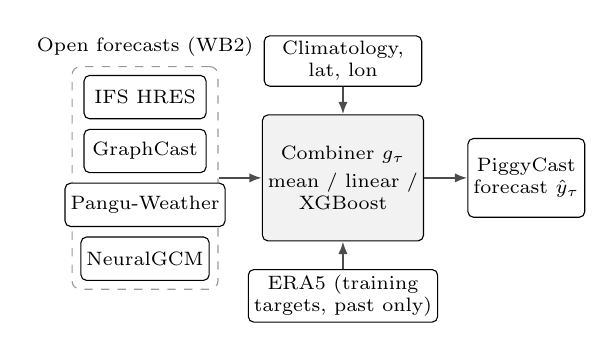
\begin{tikzpicture}[
  font=\scriptsize,
  box/.style={draw, rounded corners=2pt, align=center, minimum height=0.55cm, inner sep=2pt, fill=white},
  arr/.style={-{Latex[length=1.6mm]}, thick, draw=black!70}]
  \node[box, minimum width=1.55cm] (ifs) {IFS HRES};
  \node[box, minimum width=1.55cm, below=0.12cm of ifs] (gc) {GraphCast};
  \node[box, minimum width=1.55cm, below=0.12cm of gc] (pg) {Pangu-Weather};
  \node[box, minimum width=1.55cm, below=0.12cm of pg] (ng) {NeuralGCM};
  \begin{scope}[on background layer]
    \node[draw=black!40, dashed, rounded corners=3pt, fit=(ifs)(ng), inner sep=3pt, label={[font=\scriptsize]above:Open forecasts (WB2)}] (base) {};
  \end{scope}
  \node[box, right=0.55cm of base, minimum width=2.0cm, minimum height=1.6cm, fill=black!5] (comb) {Combiner $g_\tau$\\[2pt]mean / linear /\\XGBoost};
  \node[box, above=0.35cm of comb, minimum width=2.0cm] (aux) {Climatology,\\lat, lon};
  \node[box, right=0.55cm of comb, minimum width=1.3cm, minimum height=1.0cm] (out) {PiggyCast\\forecast $\hat{y}_\tau$};
  \node[box, below=0.35cm of comb, minimum width=2.0cm] (era) {ERA5 (training\\targets, past only)};
  \draw[arr] (base) -- (comb);
  \draw[arr] (aux) -- (comb);
  \draw[arr] (era) -- (comb);
  \draw[arr] (comb) -- (out);
\end{tikzpicture}
\caption{The PiggyCast framework. Archived forecasts from existing models are combined by a lightweight statistical model, fit separately at each lead time $\tau$ on past ERA5 verification.}\label{f:schematic}
\end{figure}

\subsection{Combiners}

We compare combiners of increasing flexibility.

\paragraph{Multi-model mean (MMM).} The equal-weight average $\bar{f}_\tau = M^{-1}\sum_m f^{(m)}_\tau$. It has no trainable parameters and is the natural baseline for any learned combiner.

\paragraph{\PCLin.} A global linear stack with climatology as an extra regressor,
\begin{equation}
\hat{y} = \textstyle\sum_{m} a_m f^{(m)}_\tau + b\, c + a_0, \label{e:lin}
\end{equation}
with six coefficients per lead time fit by area-weighted least squares. The weights are unconstrained. A climatology weight $b>0$ lets the model shrink its forecast toward climatology, which is RMSE-optimal when skill is low (section~4c and Appendix~C). We also report the same stack without the climatology term (``Linear'').

\paragraph{Per-grid-point linear stack.} A superensemble-style regression \citep{krishnamurti1999superensemble} fit independently at each of the 2048 grid points on anomalies, $y-c = \sum_m a_m(\mathbf{x})(f^{(m)}_\tau-c)+a_0(\mathbf{x})$, with a small ridge penalty (10$^{-3}$ times the mean diagonal of the Gram matrix) for numerical stability.

\paragraph{\PCXGB.} The gradient-boosted tree model of the original PiggyCast \citep{chen2016xgboost}, which predicts $y$ from the four forecasts plus latitude and longitude, with XGBoost default hyperparameters (100 trees, maximum depth 6, learning rate 0.3) and area-weighted samples, as in the original study. Appendix~E tests whether tuning changes the results. We also report a variant without latitude and longitude.

\paragraph{\PCXGBR.} A residual reformulation: the same tree model predicts the correction $y-\bar{f}_\tau$ from each model's deviation from the mean, $f^{(m)}_\tau-\bar{f}_\tau$, the mean anomaly $\bar{f}_\tau-c$, latitude, and longitude. The forecast is $\bar{f}_\tau$ plus the predicted correction. This removes the large, spatially varying absolute level of \Zfive{} from what the trees must represent.

\subsection{Leakage-safe rolling-origin evaluation}

Samples are ordered by valid time, and the evaluation must respect causality \citep{bergmeir2018cv, cerqueira2020evaluating, roberts2017cv}. We use 10 rolling-origin folds. Each fold tests on 30 consecutive days (60 valid times) and trains on the preceding 60 days (120 valid times), separated by a gap. The ten test windows tile the last 300 days of the period (8 March 2020 to 1 January 2021) and are identical for all methods and lead times.

The gap matters because the samples are indexed by valid time. A test forecast valid at $t$ with lead $\tau$ was issued at $t-\tau$. Every training target must therefore be verified before $t-\tau$, or the model trains on information that would not exist operationally. The original PiggyCast used a fixed 5-day gap, which violates this for $\tau>120$\,h. We therefore set the gap to 5 days plus the lead time, which keeps a 5-day buffer against autocorrelation. Appendix~A compares the two protocols.

\subsection{Verification}

All scores are area weighted with $w(\phi)=\cos\phi$ at latitude $\phi$. The headline score is the area-weighted RMSE over each test fold, averaged over the 10 folds:
\begin{equation}
\mathrm{RMSE} = \sqrt{\frac{\sum_{i} w_i\,(\hat{y}_i-y_i)^2}{\sum_i w_i}},
\end{equation}
where $i$ runs over all grid points and valid times in the fold. Because RMSE rewards smooth forecasts as predictability is lost, we also report the WB2 anomaly correlation coefficient (ACC; per valid time, then averaged) and the activity ratio, defined as the area-weighted root-mean-square forecast anomaly divided by that of ERA5 (per valid time, then averaged). An activity ratio below 1 indicates a forecast smoother than reality.

To test whether two methods differ, we compute the RMSE difference over all 600 test valid times and a 95\% confidence interval from a moving-block bootstrap \citep{kunsch1989bootstrap} with 5-day blocks and 2000 resamples. This accounts for the serial correlation of daily errors.

\subsection{Error structure and interpretability}

To characterize how the base models relate, we compute the area-weighted Pearson correlation between their error fields $e^{(m)}=f^{(m)}-y$ over all valid times and grid points. Following the original PiggyCast analysis, we also compute pairwise area-weighted RMSE between all model fields and ERA5. We summarize these with average-linkage (UPGMA) hierarchical clustering \citep{mullner2011clustering} and metric multidimensional scaling \citep[MDS;][]{borg2005mds}. We interpret \PCLin{} directly through its coefficients in (\ref{e:lin}), and \PCXGB{} through the area-weighted mean absolute TreeSHAP value of each input on test data \citep{lundberg2017shap, lundberg2020treeshap}.

%%%%%%%%%%%%%%%%%%%%%%%%%%%%%%%%%%%%%%%%%%%%%%%%%%%%%%%%%%%%%%%%%%%%%%
\section{Results}

\subsection{The base models make partly independent errors}

\begin{figure*}[t]
\centering
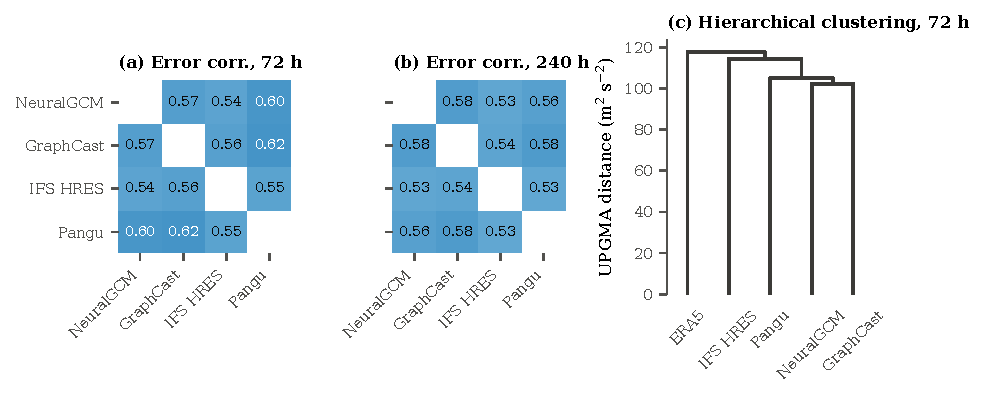
\includegraphics[width=39pc]{figures/fig_error_structure.pdf}
\caption{Error structure of the base models. (a, b) Area-weighted correlation between the error fields of each pair of base models at 72 and 240\,h lead time. (c) Average-linkage hierarchical clustering of the pairwise RMSE between model fields and ERA5 at 72\,h.}\label{f:errors}
\end{figure*}

The pairwise error correlations lie between 0.53 and 0.62 at both 72 and 240\,h (Fig.~\ref{f:errors}a,b). GraphCast and Pangu-Weather, both purely data-driven and trained on ERA5, share the most error (0.62 at 72\,h). IFS HRES, the only physics-based model, is the least correlated with the others. No pair is close to redundant. The pairwise RMSE matrix shows the same picture: at 72\,h the five fields (four models and ERA5) are nearly equidistant, with distances of 102--126\,\units{} (Fig.~\ref{f:errors}c). NeuralGCM and GraphCast are slightly closer to each other (102.4\,\units) than NeuralGCM is to ERA5 (104.4\,\units), so they merge first in the dendrogram.

This near-simplex geometry is what partly correlated errors imply. If $M$ models have equal error variance $\sigma^2$ and pairwise error correlation $\rho$, two models are separated by RMSE $\sigma\sqrt{2(1-\rho)}\approx0.95\sigma$ for $\rho=0.55$, almost the same as each model's distance $\sigma$ from the truth. The geometry also means a two-dimensional MDS embedding distorts the distances substantially: Kruskal stress-1 is 0.21 for the five fields at 72\,h and 0.24 for all 41 fields across lead times. We therefore do not interpret features of the MDS trajectories, such as the S-shape reported in the original PiggyCast analysis.

Moderate error correlation has a direct, quantitative consequence. Under the same idealization, the equal-weight mean has error variance
\begin{equation}
\sigma^2_{\bar f} = \sigma^2\,\frac{1+(M-1)\bar\rho}{M}. \label{e:mmm}
\end{equation}
With $\bar\rho = 0.57$ at 72\,h and 0.55 at 240\,h, (\ref{e:mmm}) predicts that the MMM RMSE is 82\% of the average single-model RMSE: 97.2\,\units{} at 72\,h and 613.4\,\units{} at 240\,h. The observed values are 97.4 and 613.0\,\units{} (Table~\ref{t:rmse}). Error cancellation alone accounts for the MMM's improvement. Appendix~C gives the general form for unequal skill and correlations.

\subsection{Stacking improves on every base model at every lead time}

\begin{table*}[t]
\caption{Area-weighted \Zfive{} RMSE (\units), averaged over 10 leakage-safe test folds (8 Mar 2020 -- 1 Jan 2021). Underlined: best base model. Bold: best overall. Climatology RMSE is 798.2\,\units{} at all lead times.}\label{t:rmse}
\begin{center}
\resizebox{\textwidth}{!}{%
\begin{tabular}{r|rrrr|r|rrr|rrr}
\hline\hline
 & \multicolumn{4}{c|}{Base models} & & \multicolumn{3}{c|}{Linear stacks} & \multicolumn{3}{c}{Tree stacks (XGBoost)} \\
Lead (h) & NeuralGCM & GraphCast & IFS HRES & Pangu & MMM & Linear & \PCLin & Per-point & \PCXGB & no lat/lon & \PCXGBR \\
\hline
24 & \underline{32.8} & 40.5 & 41.3 & 42.7 & 32.3 & 29.6 & 29.6 & 29.8 & 45.7 & 45.0 & \textbf{29.4} \\
48 & \underline{60.7} & 69.6 & 74.2 & 75.7 & 57.1 & 54.4 & \textbf{54.4} & 55.6 & 64.5 & 63.9 & 55.3 \\
72 & \underline{105.1} & 115.6 & 125.2 & 125.8 & 97.4 & 94.5 & \textbf{94.5} & 98.2 & 102.7 & 100.8 & 97.3 \\
96 & \underline{169.5} & 179.8 & 197.7 & 196.3 & 154.9 & \textbf{151.9} & 152.0 & 159.3 & 161.1 & 157.3 & 157.8 \\
120 & \underline{252.7} & 263.2 & 289.5 & 286.1 & 228.3 & 225.5 & \textbf{225.4} & 238.1 & 237.2 & 231.3 & 234.7 \\
144 & \underline{348.1} & 359.6 & 393.4 & 388.1 & 310.9 & 308.3 & \textbf{307.6} & 326.1 & 325.7 & 315.5 & 322.7 \\
168 & \underline{451.9} & 460.6 & 502.8 & 494.6 & 397.5 & 395.3 & \textbf{393.1} & 417.7 & 421.8 & 403.7 & 413.1 \\
192 & \underline{555.9} & 558.4 & 607.6 & 596.9 & 479.6 & 477.7 & \textbf{473.0} & 503.7 & 514.8 & 487.3 & 497.6 \\
216 & \underline{650.5} & 651.6 & 700.1 & 688.9 & 552.9 & 551.7 & \textbf{543.5} & 579.1 & 596.0 & 562.9 & 573.3 \\
240 & \underline{731.1} & 731.9 & 778.3 & 765.9 & 613.0 & 612.6 & \textbf{600.6} & 640.9 & 662.7 & 626.2 & 636.2 \\
\hline
\end{tabular}}
\end{center}
\end{table*}

\begin{figure*}[t]
\centering
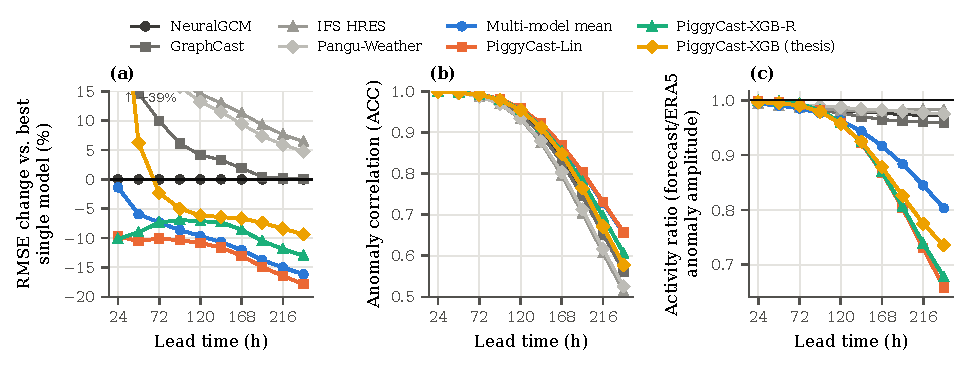
\includegraphics[width=39pc]{figures/fig_skill_vs_lead.pdf}
\caption{Skill as a function of lead time. (a) RMSE relative to the best single base model (NeuralGCM at every lead time); negative is better. \PCXGB{} at 24\,h (+39\%) is off the scale. (b) Anomaly correlation coefficient. (c) Activity ratio: the root-mean-square forecast anomaly relative to ERA5's. Values below 1 indicate a forecast smoother than reality. Gray: base models; colors: combiners. Full values are in Table~\ref{t:rmse}.}\label{f:skill}
\end{figure*}

Table~\ref{t:rmse} and Fig.~\ref{f:skill} summarize the main results. NeuralGCM is the best base model at every lead time, followed by GraphCast, which converges with it after about 7 days. \PCLin{} reduces RMSE relative to NeuralGCM by 9.7\% at 24\,h, 10.1\% at 72\,h, 13.0\% at 168\,h, and 17.9\% at 240\,h. The block-bootstrap confidence intervals exclude zero at every lead time (Table~\ref{t:boot}). It is also the best or within 0.1\,\units{} of the best method at every lead time except 24\,h, where \PCXGBR{} is marginally better (29.4 versus 29.6\,\units). The improvement is not confined to a region: \PCLin{} has lower grid-point RMSE than NeuralGCM over 97\% of the globe (by area) at 72\,h and 99.9\% at 240\,h, with the largest relative gains in the extratropics (Fig.~\ref{f:maps}a,b).

Figure~\ref{f:linbase} compares \PCLin{} directly with each base model over the full 10-day range. It reduces RMSE by 10--18\% relative to NeuralGCM, 14--27\% relative to GraphCast, 22--29\% relative to IFS HRES, and 20--31\% relative to Pangu-Weather (Fig.~\ref{f:linbase}b). Against the three HRES-initialized models the reduction is largest on day 1, partly because those models start from the operational analysis while verification is against ERA5, and it settles at 14--23\% from day 4 onward. Against NeuralGCM it grows steadily with lead time. In terms of anomaly correlation, \PCLin{} at day 10 (0.657) matches NeuralGCM at day 9 (0.656), a gain of about one day of useful predictability (Fig.~\ref{f:linbase}c). The gains are geographically uniform (Fig.~\ref{f:linbasemaps}). Over all 40 combinations of base model and lead time, \PCLin{} has lower grid-point RMSE over at least 93\% of the globe, and over at least 99\% for every combination except NeuralGCM on days 1--3. It is worse than NeuralGCM on day 1 only in small regions over the subtropical eastern North Pacific off Mexico, equatorial Africa, and part of East Antarctica, by up to 23\%. In these regions NeuralGCM is much more accurate than the other three models (their day-1 RMSE is 26--51\% higher off Mexico), so the single set of global weights, which gives NeuralGCM 0.59, under-weights it locally. Regionally varying weights (Appendix~D, item 7) could address this. Relative to IFS HRES and Pangu-Weather, the largest gains are in the tropics at days 5 and 10.

\begin{figure*}[t]
\centering
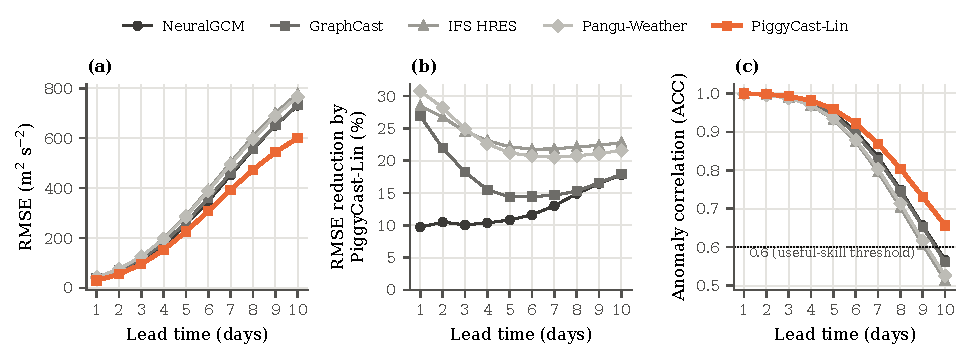
\includegraphics[width=39pc]{figures/fig_lin_vs_base.pdf}
\caption{\PCLin{} against each base model over lead times of 1--10 days. (a) Area-weighted RMSE. (b) RMSE reduction achieved by \PCLin{} relative to each base model. (c) Anomaly correlation coefficient; the dotted line marks 0.6, a common threshold for useful skill. Leakage-safe folds; test period 8 Mar 2020 -- 1 Jan 2021.}\label{f:linbase}
\end{figure*}

\begin{figure*}[t]
\centering
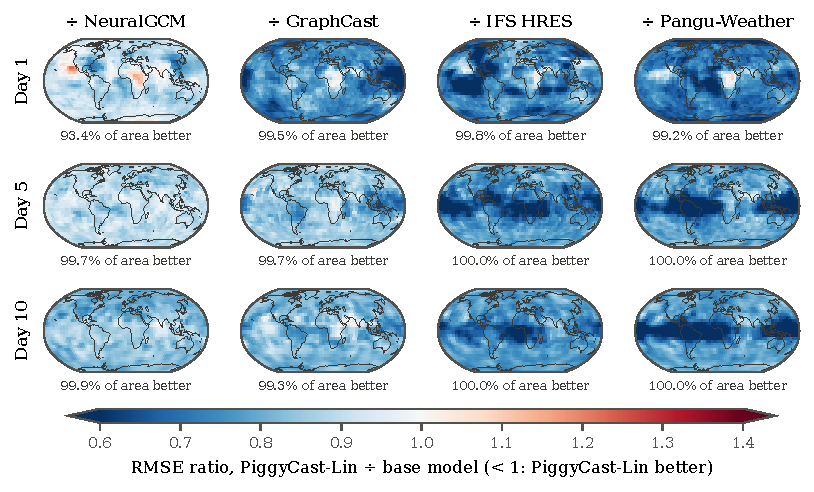
\includegraphics[width=39pc]{figures/fig_lin_vs_base_maps.pdf}
\caption{Ratio of the grid-point RMSE of \PCLin{} to that of each base model (columns) at lead times of 1, 5, and 10 days (rows), over all test valid times. Blue: \PCLin{} better. The fraction of the globe (by area) where \PCLin{} is better is given below each map.}\label{f:linbasemaps}
\end{figure*}

The equal-weight MMM captures most of this gain. It is 1.4\% better than NeuralGCM at 24\,h, rising to 7.3\% at 72\,h and 16.2\% at 240\,h. Learning weights (Linear) adds a further 3--8\% at lead times up to 72\,h, where NeuralGCM is clearly superior and deserves extra weight. The benefit of learned weights shrinks with lead time and is not significant at 240\,h (0.1\%, Table~\ref{t:boot}). Adding climatology (\PCLin) helps only at long lead times, where it contributes a further 2\% at 240\,h.

Flexibility does not help. The per-grid-point linear stack, with 10{,}240 coefficients fit to 120 training times, is worse than the global stack at every lead time and worse than the MMM beyond 48\,h. The original \PCXGB{} is worse than the MMM at every lead time, by 4--8\% beyond 72\,h and by more than 40\% at 24\,h. At 24 and 48\,h it is even worse than NeuralGCM alone (+39\% and +6\%), and it overtakes NeuralGCM only from 72\,h onward. The maps show where it loses (Fig.~\ref{f:maps}c). At 240\,h \PCXGB{} is 32\% worse than the MMM poleward of 60$^\circ$N and 10\% worse poleward of 60$^\circ$S, but 7\% better in the tropics, where it damps more strongly toward climatology. Recasting the trees as a correction to the MMM (\PCXGBR) removes the short-lead failure and makes the tree model competitive at 24--48\,h. Beyond 72\,h it is still slightly worse than the MMM. Removing latitude and longitude from \PCXGB{} improves it at every lead time beyond 24\,h (Table~\ref{t:rmse}), which indicates that the coordinates are being used to overfit.

\begin{table}[t]
\caption{RMSE change (\%) and 95\% moving-block-bootstrap confidence interval for the absolute RMSE difference (\units) of selected method pairs. Pooled over all 600 test valid times.}\label{t:boot}
\begin{center}
\small\setlength{\tabcolsep}{4pt}
\resizebox{\columnwidth}{!}{%
\begin{tabular}{rrrrr}
\hline\hline
Lead & \multicolumn{2}{c}{\PCLin{} vs NeuralGCM} & \PCXGB{} vs & Linear vs \\
(h) & \% & 95\% CI & MMM (\%) & MMM (\%) \\
\hline
24 & $-9.7$ & [$-3.3$, $-3.1$] & $+45.0$ & $-8.3$ \\
72 & $-10.1$ & [$-11.4$, $-9.9$] & $+5.7$ & $-2.9$ \\
120 & $-10.8$ & [$-30.1$, $-25.1$] & $+3.9$ & $-1.2$ \\
168 & $-13.0$ & [$-63.5$, $-54.5$] & $+6.2$ & $-0.6$ \\
240 & $-17.9$ & [$-137.8$, $-123.6$] & $+8.2$ & $-0.1^{\ast}$ \\
\hline
\end{tabular}}
\end{center}
\footnotesize{$^{\ast}$Not significant (CI includes zero). All other entries in the table are significant at the 5\% level.}
\end{table}

\begin{figure*}[t]
\centering
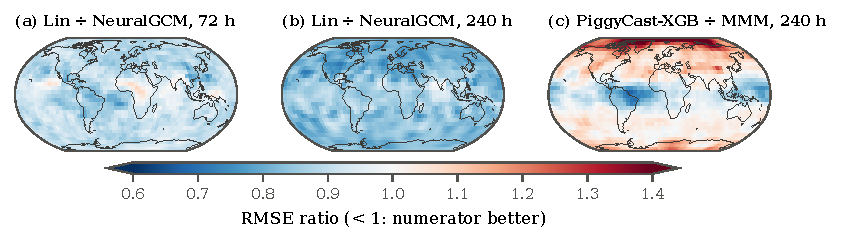
\includegraphics[width=39pc]{figures/fig_maps.pdf}
\caption{Ratio of grid-point RMSE over all test valid times. (a, b) \PCLin{} relative to NeuralGCM at 72 and 240\,h. (c) \PCXGB{} relative to the multi-model mean (MMM) at 240\,h. Blue: numerator better.}\label{f:maps}
\end{figure*}

\subsection{At long lead times, part of the gain is damping}

Skill gains measured by RMSE can come from a better forecast or from a smoother one. ACC is insensitive to amplitude, and it shows that the stacked forecasts are genuinely better at placing anomalies. \PCLin{} raises ACC from 0.835 (NeuralGCM) to 0.869 at 168\,h and from 0.566 to 0.657 at 240\,h (Fig.~\ref{f:skill}b). The MMM achieves almost the same ACC (0.867 and 0.655), as expected, since a uniform rescaling of anomalies leaves ACC unchanged.

The activity ratio, however, falls steeply for all combiners (Fig.~\ref{f:skill}c). The base models keep realistic variability (0.96--0.98 at 240\,h), whereas the MMM's anomalies are 20\% too weak at 240\,h because averaging cancels unpredictable features. \PCLin{} goes further, to 0.66. This is not a failure of the stack but the RMSE-optimal response to limited skill. For a forecast with anomaly correlation $r$, the mean squared error is minimized when the forecast anomaly amplitude is $r$ times the observed one \citep{murphy1988skill}. \PCLin{} meets this condition almost exactly: its activity ratio equals its ACC to two decimals at 168\,h (0.869 versus 0.869) and 240\,h (0.66 versus 0.657). The tree-based stacks show the same damping. Figure~\ref{f:case} illustrates it for a single strong Northern Hemisphere winter case. The 240-h NeuralGCM forecast has realistic anomaly amplitudes but misplaces several features. The multi-model mean keeps the large-scale pattern with weaker anomalies, and \PCLin{} damps them further. In this particular case damping beyond the mean is not rewarded: \PCLin{} has a higher Northern Hemisphere RMSE (998\,\units) than the mean (939\,\units), although it is lower on average over all test cases. The large gains over IFS HRES reported for the original \PCXGB{} at day 10 (about 16\%) therefore mix genuine skill with smoothing. Users who need realistic variability, for example for extremes, should account for this (section~5).

\begin{figure*}[t]
\centering
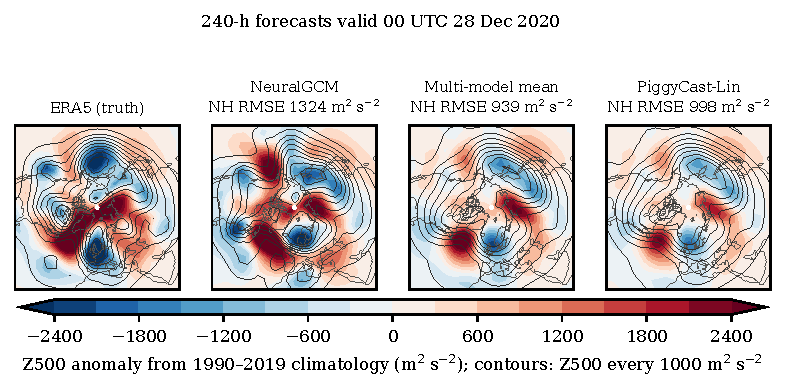
\includegraphics[width=39pc]{figures/fig_case_study.pdf}
\caption{Case study: 240-h \Zfive{} forecasts valid 0000 UTC 28 December 2020 (initialized 18 December), the test case from November--December with the largest Northern Hemisphere extratropical anomaly. Shading: anomaly from the 1990--2019 ERA5 climatology. Contours: \Zfive{} every 1000\,\units. RMSE is area weighted over 30--90$^\circ$N. \PCLin{} is trained on the corresponding leakage-safe fold.}\label{f:case}
\end{figure*}

\subsection{What the stacks learn}

\begin{figure}[t]
\centering
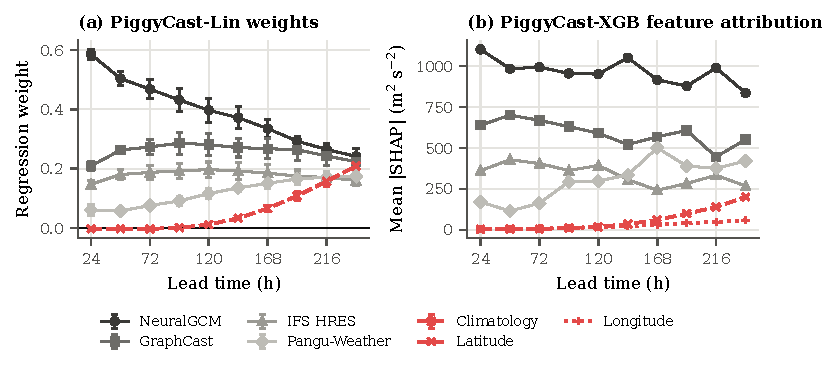
\includegraphics[width=19pc]{figures/fig_weights_shap.pdf}
\caption{What the stacks learn. (a) \PCLin{} regression weights, mean $\pm$1 standard deviation across the 10 folds. (b) Area-weighted mean absolute SHAP value of each \PCXGB{} input on test data (folds 1, 5, and 10).}\label{f:weights}
\end{figure}

The \PCLin{} weights are stable across folds and tell a simple story (Fig.~\ref{f:weights}a). At 24\,h NeuralGCM receives a weight of 0.59, GraphCast 0.21, IFS HRES 0.15, and Pangu-Weather 0.06, roughly in order of individual skill. As lead time increases the weights converge toward equality (0.16--0.24 at 240\,h), which matches the convergence of the base models' RMSE. At the same time, the climatology weight grows from zero at 72\,h to 0.21 at 240\,h. The model weights sum to about 1 at short lead times and to $1-b$ at long ones, so the stack is an explicit, skill-dependent blend between the multi-model forecast and climatology.

The SHAP attributions of \PCXGB{} are consistent with this but harder to read (Fig.~\ref{f:weights}b). NeuralGCM is the most important input at every lead time, and Pangu-Weather the least important at short lead times. The attribution to latitude rises from 3\,\units{} at 24\,h to 201\,\units{} at 240\,h. The earlier PiggyCast analysis read this as a growing role for ``spatial anchoring''. Our results suggest a more specific interpretation: climatology varies strongly with latitude, so latitude is the tree model's proxy for the damping toward climatology that \PCLin{} represents explicitly through $b$. The same flexibility lets the trees fit spurious location-specific structure, which is why removing the coordinates improves the forecasts (Table~\ref{t:rmse}).

\subsection{Sensitivity to training length}

\begin{figure*}[t]
\centering
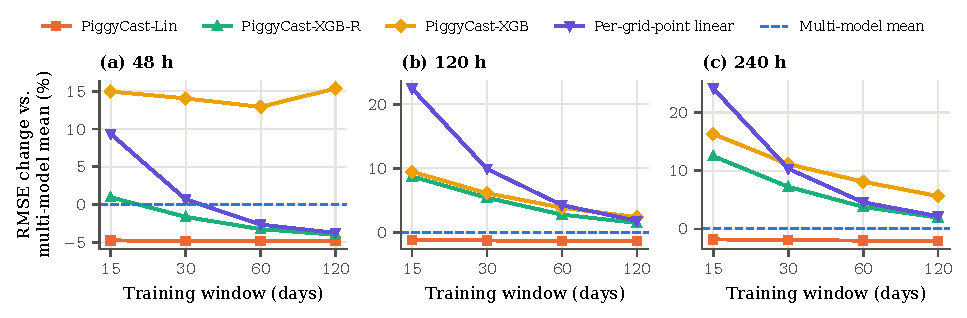
\includegraphics[width=39pc]{figures/fig_trainlen.pdf}
\caption{Sensitivity to the length of the training window at 48, 120, and 240\,h lead time, expressed as RMSE relative to the multi-model mean (dashed, which needs no training). Leakage-safe folds; test windows as in Table~\ref{t:rmse}.}\label{f:trainlen}
\end{figure*}

Figure~\ref{f:trainlen} varies the training window from 15 to 120 days. \PCLin{} is essentially insensitive: 15 days of training (30 valid times, about 60{,}000 grid-point samples for six coefficients) give the same skill as 120 days. The flexible combiners improve steadily with more data. With 120 days, \PCXGBR{} and the per-grid-point stack approach, but do not reach, the MMM at 120 and 240\,h. This suggests that they could become useful with multi-year training archives, but at the data scale of a single verification year they are dominated by the linear stack. Appendix~E tests this with up to two years of training data for two- and three-model stacks: the long-lead gap closes, but the tree stacks still do not overtake \PCLin{}.

\subsection{Computational cost}

Fitting \PCLin{} for all 10 lead times and 10 folds takes under a second on a laptop CPU (0.08\,s per lead time). The main experiment (all combiners, folds, lead times, and both gap protocols) runs in about three minutes on a 12-core laptop without a GPU. The cost of a PiggyCast forecast is negligible compared with that of running any one of the base models, let alone training it.

%%%%%%%%%%%%%%%%%%%%%%%%%%%%%%%%%%%%%%%%%%%%%%%%%%%%%%%%%%%%%%%%%%%%%%
\section{Discussion}

\paragraph{Why stacking works here.} The gains decompose cleanly. Most of the improvement comes from averaging models whose errors are only moderately correlated, which (\ref{e:mmm}) predicts to within a fraction of a percent. Learned weights add a few percent at short lead times, where one model is clearly better. At long lead times the stack learns the RMSE-optimal damping toward climatology. None of these mechanisms needs a nonlinear learner. This mirrors the experience with NWP multimodel ensembles \citep{krishnamurti1999superensemble, hagedorn2005multimodel} and is consistent with recent work combining AIWP models, where simple averaging is a strong baseline \citep{chakraborty2025mowe, weyn2024ensemble}. Model diversity, not combiner complexity, is the main ingredient.

\paragraph{Why the tree stack struggles.} XGBoost approximates the target with a sum of piecewise-constant functions. The combiner essentially needs to represent a near-identity map of absolute \Zfive{}, a quantity spanning almost 15{,}000\,\units{} (44{,}100--58{,}800\,\units{} in our data). With 100 depth-6 trees this leaves an approximation error that is negligible at 10 days but comparable to the entire forecast error at 1 day: at 24\,h the training-set RMSE is already 39.6\,\units{}, above NeuralGCM's test error, so the problem is underfitting rather than overfitting. This explains the poor short-range result of the original PiggyCast. Learning the residual from the MMM removes this level. The remaining gap at long lead times reflects variance from fitting a flexible model to about 120 strongly autocorrelated training days. Nested hyperparameter tuning (Appendix~E) reduces this gap when training data are scarce, mainly by choosing shallower trees and fewer boosting rounds, but it does not change the ranking. The multi-year experiment in Appendix~E supports both parts of this explanation. Two years of training data close most of the long-lead gap, whereas the 24-h deficit of \PCXGB{} remains near 30\% and does not change with 500 deeper trees.

\paragraph{The evaluation protocol matters.} With the original 5-day gap, the training set at lead times beyond 120\,h contains verifying analyses that postdate the issue time of the test forecasts. For the linear stacks this changes RMSE by less than 0.1\%, but for \PCXGB{} it flatters the score by up to 2.4\% at 240\,h (Appendix~A). The flexible model benefits most from the leaked information, so stacking studies should use a gap of at least the lead time.

\paragraph{RMSE and smooth forecasts.} RMSE-optimal stacks are necessarily smoother than reality at long lead times. This is appropriate for a deterministic best estimate but not for applications that need realistic variability or extremes. Probabilistic stacking, for example ensemble model output statistics or Bayesian model averaging \citep{gneiting2005emos, raftery2005bma, vannitsem2021postprocessing}, or neural post-processing with proper scores \citep{rasp2018postprocessing}, would provide calibrated uncertainty instead of damped means. It is the natural next step for PiggyCast.

\paragraph{Limitations.} Our evaluation covers one variable, one coarse resolution (5.625$^\circ$), and one year, which is the overlap currently available for all four models in WB2. NeuralGCM and operational GraphCast forecasts are archived only for 2020. The test period does not include a full annual cycle of out-of-sample training, and results may differ at higher resolution, for surface variables, or for extremes. The base models are verified against ERA5, which slightly disadvantages IFS HRES at short lead times, and NeuralGCM is initialized from ERA5 rather than an operational analysis. Because the stacks are trained on archived forecasts, operational use would require that the base models' forecast distributions remain stable. A model upgrade would require retraining, although the 15-day data requirement of \PCLin{} makes this cheap. Appendix~E repeats the comparison over 2020--2022 for the subsets of models archived in those years, and Appendix~D lists the remaining experiments needed to test how far the conclusions generalize.

%%%%%%%%%%%%%%%%%%%%%%%%%%%%%%%%%%%%%%%%%%%%%%%%%%%%%%%%%%%%%%%%%%%%%%
\section{Conclusions}

We have presented PiggyCast, a framework for stacking the openly released forecasts of numerical, AI, and hybrid weather models. For 500-hPa geopotential at lead times of 1--10 days, a six-parameter linear stack reduces RMSE by 10--18\% and raises ACC relative to the best single model, needs about two weeks of training data, and costs seconds to fit. Most of this improvement comes from averaging models with moderately correlated errors, and at long lead times the remainder comes from RMSE-optimal damping toward climatology. A gradient-boosted tree combiner, used in earlier versions of this work, adds no value at this data scale and harms short-range forecasts unless it is reformulated to learn a residual. As the number of openly available frontier forecasts grows, stacking them offers researchers and forecasting centres with limited compute a simple and robust way to obtain a forecast better than any single model. Future work should extend PiggyCast to more variables, higher resolution, multi-year training archives, and probabilistic combination.

%%%%%%%%%%%%%%%%%%%%%%%%%%%%%%%%%%%%%%%%%%%%%%%%%%%%%%%%%%%%%%%%%%%%%%
\acknowledgments
This work builds on J.~K.~Kimani's MSc research at AIMS South Africa, supervised by O.~Ang\'elil and C.~Toumping Fotso (Ishango.ai); S.~Knoblauch joined the work for the Climate Change AI tutorial at NeurIPS 2025 and the CCAI Summer School 2026. We thank AIMS South Africa and its sponsors for supporting this work, and the WeatherBench~2 team for making forecast archives and evaluation tools openly available. We thank the organizers and participants of the Climate Change AI tutorials at NeurIPS 2025 and the CCAI Summer School 2026 for feedback on earlier versions of PiggyCast.

\datastatement
All data are publicly available from the WeatherBench~2 archive (\url{https://weatherbench2.readthedocs.io}, bucket \url{gs://weatherbench2/datasets/}): ERA5 (\url{era5/1959-2023_01_10-6h-64x32_equiangular_conservative.zarr}), ERA5 climatology (\url{era5-hourly-climatology/1990-2019_6h_64x32_equiangular_conservative.zarr}), IFS HRES (\url{hres/2016-2022-0012-64x32_equiangular_conservative.zarr}), GraphCast (\url{graphcast_hres_init/2020/date_range_2019-11-16_2021-02-01_12_hours-64x32_equiangular_conservative.zarr}), Pangu-Weather (\url{pangu_hres_init/2020_0012_64x32_equiangular_conservative.zarr}), and NeuralGCM (\url{neuralgcm_deterministic/2020-64x32_equiangular_conservative.zarr}). Code to reproduce all experiments and figures (\texttt{experiments/}, one command: \texttt{./run\_all.sh}) is available at \url{https://github.com/josiahkim29/PiggyCast}.

%%%%%%%%%%%%%%%%%%%%%%%%%%%%%%%%%%%%%%%%%%%%%%%%%%%%%%%%%%%%%%%%%%%%%%
\appendix[A]
\appendixtitle{Effect of the Train--Test Gap}

Table~\ref{t:gap} compares the original fixed 5-day gap with the leakage-safe gap of 5 days plus the lead time. The test windows are identical, so only the training windows differ. The linear stack is unaffected. \PCXGB{} is increasingly flattered by the shorter gap as lead time grows, by up to 15.8\,\units{} (2.4\%) at 240\,h.

\begin{table}[h]
\caption{Fold-mean RMSE (\units) with the original 5-day gap and with the leakage-safe gap (5 days + lead time).}\label{t:gap}
\begin{center}
\small\setlength{\tabcolsep}{3.5pt}
\resizebox{\columnwidth}{!}{%
\begin{tabular}{rr|rr|rr|rr}
\hline\hline
Lead & Safe gap & \multicolumn{2}{c|}{\PCLin} & \multicolumn{2}{c|}{\PCXGB} & \multicolumn{2}{c}{\PCXGBR} \\
(h) & (days) & 5 d & safe & 5 d & safe & 5 d & safe \\
\hline
24 & 6 & 29.6 & 29.6 & 45.4 & 45.7 & 29.4 & 29.4 \\
48 & 7 & 54.4 & 54.4 & 64.4 & 64.5 & 55.3 & 55.3 \\
72 & 8 & 94.5 & 94.5 & 101.9 & 102.7 & 97.2 & 97.3 \\
96 & 9 & 151.9 & 152.0 & 159.9 & 161.1 & 157.5 & 157.8 \\
120 & 10 & 225.3 & 225.4 & 237.0 & 237.2 & 234.7 & 234.7 \\
144 & 11 & 307.6 & 307.6 & 324.9 & 325.7 & 322.5 & 322.7 \\
168 & 12 & 393.0 & 393.1 & 419.0 & 421.8 & 412.8 & 413.1 \\
192 & 13 & 472.8 & 473.0 & 506.8 & 514.8 & 496.7 & 497.6 \\
216 & 14 & 543.2 & 543.5 & 583.8 & 596.0 & 572.2 & 573.3 \\
240 & 15 & 600.2 & 600.6 & 646.9 & 662.7 & 633.1 & 636.2 \\
\hline
\end{tabular}}
\end{center}
\end{table}

\appendix[B]
\appendixtitle{Reproduction of the Original PiggyCast Results}

The original study used the valid-time window 4 January 2020 to 4 January 2021 and a GPU implementation of XGBoost. Rerunning \PCXGB{} at 72\,h on that window with the original 5-day gap gives a fold-mean RMSE of 101.8\,\units, compared with 101.99 reported originally (the difference is consistent with CPU versus GPU histogram construction). The base-model RMSEs (NeuralGCM 105.1, GraphCast 115.5, IFS HRES 125.0, Pangu-Weather 125.8\,\units) match the original values and those published by WB2. The original analysis reported \Zfive{} errors in meters. The WB2 variable is geopotential, so these values are in \units.

\appendix[C]
\appendixtitle{Mathematical Details}

\subsection{Notation}

For a fixed lead time $\tau$, index samples by $i=(\mathbf{x},t)$ and let $\langle\cdot\rangle$ denote the average over a set of samples weighted by $w_i=\cos\phi_i$. Base-model errors are $e_m=f^{(m)}_\tau-y$, with mean squared error $\sigma_m^2=\langle e_m^2\rangle$ and uncentred error correlation $\rho_{mn}=\langle e_m e_n\rangle/(\sigma_m\sigma_n)$, as in Fig.~\ref{f:errors}. Anomalies are departures from climatology, $f'=f-c$ and $y'=y-c$.

\subsection{Error of the multi-model mean}

The error of the equal-weight mean is the mean of the errors, $\bar e=M^{-1}\sum_m e_m$, so without any further assumption
\begin{equation}
\mathrm{MSE}(\bar f)=\frac{1}{M^2}\sum_{m=1}^{M}\sum_{n=1}^{M}\rho_{mn}\,\sigma_m\sigma_n. \label{e:mmmgen}
\end{equation}
Equation~(\ref{e:mmm}) is the special case $\sigma_m=\sigma$, $\rho_{mn}=\bar\rho$ for $m\neq n$. Evaluating (\ref{e:mmmgen}) with each model's own pooled RMSE and the correlations of Fig.~\ref{f:errors} gives 97.3 and 614.4\,\units{} at 72 and 240\,h, against observed pooled values of 97.5 and 614.0\,\units. The small differences arise because the correlations are estimated over the whole common window and the RMSEs over the test windows only.

The mean beats model $k$ when (\ref{e:mmmgen}) is smaller than $\sigma_k^2$. Unequal skill makes this harder. For two models with $\sigma_2=\kappa\sigma_1$, $\kappa\ge1$, the mean beats the better model only if
\begin{equation}
\rho<\frac{3-\kappa^2}{2\kappa}. \label{e:twomodel}
\end{equation}
At 24\,h the other models' RMSEs are 1.23--1.30 times NeuralGCM's. With $\kappa=1.25$ the bound is $\rho<0.58$, close to the error correlations of 0.53--0.62 observed at 72 and 240\,h. This explains why the MMM barely improves on NeuralGCM at 24\,h (1.4\%), while learned weights, which can favor the better model, gain 10\%.

\subsection{The linear stack generalizes the mean}

Write (\ref{e:lin}) as $\hat{\mathbf y}=\mathbf X\boldsymbol\theta$, where the columns of $\mathbf X$ are the $M$ forecasts, the climatology, and a constant, and let $\mathbf W=\mathrm{diag}(w_i)$. The weighted least squares estimate is
\begin{equation}
\hat{\boldsymbol\theta}=(\mathbf X^{\mathsf T}\mathbf W\mathbf X)^{-1}\mathbf X^{\mathsf T}\mathbf W\mathbf y. \label{e:wls}
\end{equation}
The MMM is the special case $\boldsymbol\theta=(M^{-1},\dots,M^{-1},0,0)$, so on its training data \PCLin{} can never be worse than the MMM. On test data it can lose only through estimation error. For $p$ parameters this error scales roughly as $\sigma^2 p/n_{\mathrm{eff}}$, where $n_{\mathrm{eff}}$ is the effective number of independent samples. With $p=6$ and about 60{,}000 strongly correlated samples even in a 15-day window, the term is negligible, which is consistent with the flat training-length curve in Fig.~\ref{f:trainlen}. The per-grid-point stack fits five parameters at each point from only 30--240 valid times, so its estimation error is much larger and decreases visibly with training length.

Rearranging (\ref{e:lin}) in anomaly form gives
\begin{equation}
\hat y-c=\sum_m a_m f'^{(m)}+\Big(\sum_m a_m+b-1\Big)c+a_0. \label{e:linanom}
\end{equation}
The fitted coefficients satisfy $\sum_m a_m+b=1.00$--$1.01$ at every lead time. The small middle term, of order 1\% of $c$, is largely offset by the intercept ($a_0$ between $-98$ and $-486$\,\units), so together they act as a bias correction. The anomaly forecast is therefore a weighted mean of the model anomalies scaled by $s=\sum_m a_m$. This factor is 1.00 up to 96\,h and falls to 0.94 at 168\,h and 0.80 at 240\,h. The climatology weight $b\approx1-s$ is the shrinkage toward climatology seen in Fig.~\ref{f:weights}a.

\subsection{Optimal damping}

Consider an anomaly forecast $f'$ with standard deviation $\sigma_f$, verifying anomalies with standard deviation $\sigma_y$, and correlation $r$. Scaling the forecast by $\alpha$ gives
\begin{equation}
\mathrm{MSE}(\alpha f')=\alpha^2\sigma_f^2-2\alpha r\sigma_f\sigma_y+\sigma_y^2,
\end{equation}
which is minimized at
\begin{equation}
\alpha^*=r\,\frac{\sigma_y}{\sigma_f},\qquad \mathrm{MSE}(\alpha^* f')=\sigma_y^2(1-r^2). \label{e:murphy}
\end{equation}
At the optimum the activity ratio $\alpha^*\sigma_f/\sigma_y$ equals $r$ \citep{murphy1988skill}. Applied to the MMM, whose ACC is $r$ and activity ratio is $A$, the optimal extra shrinkage is $\alpha^*=r/A$. This is 0.945 at 168\,h and 0.816 at 240\,h. The shrinkage that \PCLin{} learns, $s$ in (\ref{e:linanom}), is 0.939 and 0.801. The two agree to within 2\%, although the ACC and activity in Fig.~\ref{f:skill} are uncentred and averaged per valid time, so the agreement is not expected to be exact.

\subsection{Leakage-safe gap}

Let a test fold begin at valid time $t_s$. Its earliest forecast at lead $\tau$ was issued at $t_s-\tau$. Operationally, every training target must be verified before that issue time. With training valid times ending at $t_s-G$ and a buffer $\delta$ against autocorrelation, this requires
\begin{equation}
G(\tau)\ge\tau+\delta. \label{e:gap}
\end{equation}
We use $\delta=5$\,days. The original fixed gap $G=5$\,days satisfies $t_s-G\le t_s-\tau$ only for $\tau\le120$\,h and leaks for all longer leads.

\subsection{Moving-block bootstrap}

For methods A and B, let $d_A(t)$ and $d_B(t)$ be the area-weighted MSE at each of the $n=600$ test valid times. A bootstrap replicate draws $\lceil n/\ell\rceil$ block starts uniformly from $\{1,\dots,n-\ell+1\}$, concatenates the blocks of length $\ell=10$ (5 days), and truncates the result to $n$ times. The same indices are used for both methods, so the test is paired. The statistic is $\Delta^*=\sqrt{\overline{d_A^*}}-\sqrt{\overline{d_B^*}}$. The 95\% interval is given by the 2.5th and 97.5th percentiles of 2000 replicates.

\subsection{Scale of the tree-model targets}

Over the common valid window, absolute \Zfive{} has an area-weighted standard deviation of 2768\,\units{} (range 44{,}137--58{,}848\,\units), and its anomaly from climatology has a standard deviation of 793\,\units. The residual from the MMM has a standard deviation of 32.2\,\units{} at 24\,h and 611\,\units{} at 240\,h. At 24\,h, \PCXGB{} must resolve differences of about 30\,\units{} in a target that varies about 86 times more. \PCXGBR{} removes this mismatch, which is why it fixes the short-range failure and helps much less at 240\,h.

\appendix[D]
\appendixtitle{Recommended Extensions and Robustness Checks}

% Note to authors: this appendix records the work needed before the conclusions can be generalized.
% Before submission, decide whether to keep it as an appendix, fold it into section 5, or move completed items into the main text.

The conclusions above rest on one variable, one year, and one coarse grid. Table~\ref{t:future} lists the experiments needed to test how far they generalize, together with what the current WB2 archive allows. Item 1 is reported in Appendix~E. Items 2 and 3 can be run with the released code by changing the data paths and the list of base models.

\begin{table*}[t]
\caption{Recommended extensions. ``Feasible in WB2'' refers to the public archive at the time of writing.}\label{t:future}
\begin{center}
\small
\begin{tabular}{>{\raggedright\arraybackslash}p{0.3cm}>{\raggedright\arraybackslash}p{3.0cm}>{\raggedright\arraybackslash}p{5.8cm}>{\raggedright\arraybackslash}p{5.4cm}}
\hline\hline
 & Extension & Question addressed & Feasible in WB2 \\
\hline
1 & Multi-year training & Does \PCXGB{} or \PCXGBR{} overtake \PCLin{} with 2--3 years of training (Fig.~\ref{f:trainlen})? & Done for two- and three-model stacks (Appendix~E); NeuralGCM is archived for 2020 only \\
2 & Higher resolution & Do the ranking and the error-correlation structure hold at 1.5$^\circ$? & Yes, all four models at 240$\times$121 \\
3 & More variables & Does the result generalize to T850, 2-m temperature, wind, and mean sea level pressure? & Yes, same archives \\
4 & Verification against analyses & Does verifying HRES-initialized models against the HRES analysis, following WB2 convention, change the weights? & Yes \\
5 & Extremes and scale-dependent skill & What does damping cost for extremes and for small-scale variance (e.g., power spectra, extreme-dependency scores)? & Yes \\
6 & Constrained and tuned combiners & Do weights constrained to sum to one or be non-negative, or nested-CV tuning of XGBoost, change the conclusions? & Tuning done (Appendix~E); constrained weights: yes \\
7 & Regime- or region-dependent weights & Do weights fit by season, region, or flow regime add skill beyond a global stack? & Yes, but needs multi-year data \\
8 & Probabilistic stacking & Can EMOS- or BMA-type combination of ensemble forecasts give calibrated uncertainty instead of damped means (CRPS)? & Partly: ensemble archives are not available for all four models \\
\hline
\end{tabular}
\end{center}
\end{table*}

\appendix[E]
\appendixtitle{Multi-Year Training Experiment}

The main experiments are limited to one year, the only period archived for all four models. To test whether the tree-based stacks need more data rather than a different design, we repeated the comparison with the models that WB2 archives over several years, at the same resolution and lead times and with the same leakage-safe gap (5\,days plus the lead time).

\paragraph{Design.} Experiment~A stacks IFS HRES and Pangu-Weather (HRES-initialized, as in the main text) over valid times from 11~January 2020 to 31~December 2022. Each calendar month of 2022 is one test fold, and the training window is the $N$ days ending one gap before the test month, with $N$ from 15 to 700 days. Experiment~B stacks IFS HRES with the ERA5-initialized Pangu-Weather and GraphCast archives. GraphCast is available only for 2018, 2020, and 2022, so March to December 2022 are the test folds. We compare training on the preceding 60 days, as in the main text, with training on 2018, 2020, and those 60 days (781 days). Both experiments use the default XGBoost settings of the main text. At the longest window, Experiment~A also fits a larger model (500 trees of depth 8, learning rate 0.05, row and column subsampling 0.8).

\begin{figure*}[t]
\centering
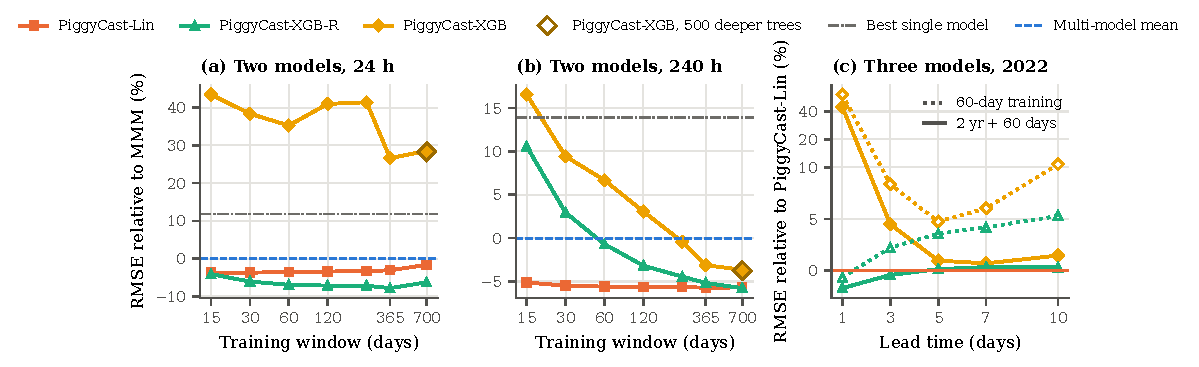
\includegraphics[width=39pc]{figures/fig_multiyear.pdf}
\caption{Multi-year training. (a,b) Experiment~A (IFS HRES and Pangu-Weather, test year 2022): RMSE relative to the two-model mean against the length of the training window at 24 and 240\,h. The open diamond is \PCXGB{} with 500 deeper trees. (c) Experiment~B (IFS HRES, Pangu-Weather, and GraphCast, ERA5-initialized; test March--December 2022): RMSE of the tree stacks relative to \PCLin{} trained on the same data, for 60-day training (dotted, open symbols) and for 2018, 2020, and 60 days (solid). Symmetric-log axis above 10\%.}\label{f:multiyear}
\end{figure*}


\paragraph{Results.} Figure~\ref{f:multiyear} summarizes four findings.
\begin{enumerate}
\item \PCLin{} does not need more data. Its RMSE changes by less than 2\% between 15 and 700 days of training, and in 2022, with 60 days of training, it is 12--17\% better than the better of the two base models at every lead time. With three models it is 9--14\% better than the best single model (GraphCast). So the main result holds for a different year and for different sets of base models.
\item At long lead times, more data closes most of the gap for \PCXGB{}. At 240\,h it moves from 6.7\% worse than the two-model mean with 60 days to 3.6\% better with 700 days, and it beats the mean in all 12 test months. It remains 2.2\% worse than \PCLin{} (1.5\% with three models and two years of training).
\item At short lead times, more data does not help \PCXGB{}. At 24\,h it is still 28\% worse than the two-model mean after 700 days of training, and the larger model gives the same result (47.9 against 48.0\,\units{}). This is the underfitting of absolute \Zfive{} described in section~5, not a lack of data.
\item \PCXGBR{} matches \PCLin{} once it has a year or more of data. With 700 days, the two agree to within 0.1\% at 120--240\,h. At 24 and 72\,h, \PCXGBR{} is 4.7\% and 0.9\% better in all 12 months. With three models it is 1.7\% and 0.4\% better, in 10 and 9 of the 10 months. With 60 days it is 1--5\% worse than \PCLin{} beyond day 1, as in the main experiment.
\end{enumerate}

\paragraph{Hyperparameter tuning.} The tree stacks above use XGBoost defaults. To test whether tuning changes the conclusions, we tuned both tree stacks in Experiment~A at 24, 120, and 240\,h with 60 and 700 days of training. The hyperparameters were chosen once per lead time and training length, using only the training window of the first test fold (data before 2022). The last 20\% of that window served as a validation block, separated from the inner training block by the leakage-safe gap. The grid crossed maximum depth (4 or 8), minimum child weight (1 or 100), and L2 penalty (1 or 50), with learning rate 0.05, row and column subsampling 0.8, and up to 2000 trees with early stopping after 50 rounds. The selected setting and number of trees were then frozen and refit in each of the 12 test months.

\begin{table}[H]
\caption{Effect of nested hyperparameter tuning (Experiment~A, test year 2022). RMSE in \units{}, mean over 12 monthly folds. XGB, XGB-R, and Lin denote \PCXGB{}, \PCXGBR{}, and \PCLin{}; default means the XGBoost defaults used in the main text.}\label{t:tuning}
\begin{center}
\footnotesize
\setlength{\tabcolsep}{4pt}
\begin{tabular}{llrrrrr}
\hline\hline
Lead & Train & \multicolumn{2}{c}{XGB} & \multicolumn{2}{c}{XGB-R} & Lin \\
 & (days) & default & tuned & default & tuned & \\
\hline
24\,h & 60 & 50.5 & 50.2 & 34.8 & 34.5 & 36.0 \\
24\,h & 700 & 48.0 & 48.1 & 35.0 & 35.0 & 36.7 \\
120\,h & 60 & 263.3 & 255.2 & 259.6 & 252.2 & 252.1 \\
120\,h & 700 & 254.0 & 253.5 & 252.3 & 251.6 & 252.4 \\
240\,h & 60 & 725.7 & 675.4 & 675.5 & 644.6 & 642.2 \\
240\,h & 700 & 655.5 & 654.2 & 641.0 & 639.2 & 641.6 \\
\hline
\end{tabular}
\end{center}
\end{table}



Tuning matters mostly with short training windows (Table~\ref{t:tuning}). With 60 days, it reduces the 240-h RMSE of \PCXGB{} by 6.9\% and of \PCXGBR{} by 4.6\%, in all 12 months. The selected models are shallow and stop early (6--124 trees at 120 and 240\,h), so tuning acts mainly as regularization, pulling the tree stacks toward the multi-model mean. With 700 days, tuning changes RMSE by 0.3\% or less. It does not fix the short-range failure of \PCXGB{}, which stays 31--39\% worse than \PCLin{} at 24\,h. Tuned \PCXGB{} remains worse than \PCLin{} in every configuration. Tuned \PCXGBR{} is tied with \PCLin{} (within 0.4\%) at 120 and 240\,h with 60 days of training. With 700 days it is 0.3--0.4\% better at those lead times (in 10 and 9 of 12 months) and 4.7\% better at 24\,h.

A nonlinear stack therefore adds clear skill only at short lead times, and only when it learns a correction to the mean. At medium range, even a tuned residual stack with two years of data improves on the six-parameter linear stack by less than half a percent. These experiments omit NeuralGCM and use a single test year, so they do not replace the four-model results in the main text.

\FloatBarrier
%%%%%%%%%%%%%%%%%%%%%%%%%%%%%%%%%%%%%%%%%%%%%%%%%%%%%%%%%%%%%%%%%%%%%%
\bibliographystyle{ametsocV6}
\bibliography{piggycast}

\end{document}
